% Provenance (never printed): see sources/outline_sources.md (Year 2: effusive and explosive
% eruptions, eruptive styles, eruption columns, pyroclastic deposits, explosivity index,
% volcano monitoring).
% Curves from figdata/bachelor-2/eruptions.py (closed-system gas fraction, Cotopaxi Layer 5
% thinning, GVP frequency-size law, column height fits, Mogi uplift); exercise and problem
% values in the Book 4 scratch calculators calc/ch06.py and calc/ch06pb.py.
\chapter{Las erupciones volcánicas}\label{ch:b2:eruptive-styles}

El 15 de junio de 1991, el monte Pinatubo, en Filipinas, expulsó más de cinco
kilómetros cúbicos de material; su nube de ceniza subió hasta
\qty{35}{km}, la cima se hundió formando una \omterm{def:b2:eruptive-styles:caldera}{caldera} de \qty{2.5}{km} de diámetro, y los
veinte millones de toneladas de dióxido de azufre que inyectó en la estratosfera enfriaron
todo el planeta cerca de medio grado durante dos años. Una semana antes, el primer
\omterm{def:b2:magma-emplacement:magma}{magma} que llegó a la superficie no había hecho nada parecido: tras perder la mayor parte de su
gas durante el ascenso, salió lentamente como un \omterm{def:b2:eruptive-styles:dome}{domo de lava}. En el Kīlauea, en Hawái, la
erupción del Pu`u~`\=O`\=o emitió \qty{4.4}{km^3} de lava, un volumen comparable,
durante treinta y cinco años, en forma de fuentes y coladas que destruyeron 215 edificios
sin levantar nunca una gran columna de ceniza. La misma Tierra, la misma física, tres comportamientos: lo que
los separa es cuánto gas lleva un \omterm{def:b2:magma-emplacement:magma}{magma}, si ese gas puede abandonar el
fundido con calma, y con qué rapidez sube el \omterm{def:b2:magma-emplacement:magma}{magma}. Este capítulo sigue una erupción
desde las burbujas del conducto hasta la columna que se alza sobre la boca y los depósitos que
deja, después mide las erupciones, las cuenta y vigila los volcanes en busca de las
señales de que se acerca una.
% ledger: usgs:pinatubo-1991, usgs:puuoo

\begin{recall}
\textbf{De los volúmenes escolares}: un volcán, su boca y su cráter, la cámara
magmática que hay debajo, la lava y la ceniza volcánica. \textbf{Del
\cref{ch:b2:magma-emplacement}}: los \omterm{def:b2:magma-emplacement:volatiles}{volátiles magmáticos}, su exsolución por debajo de la
presión de saturación, la ley de la raíz cuadrada de la solubilidad del agua, $w = s\sqrt p$, con
$s \approx 0.34$ por ciento por $\sqrt{\unit{MPa}}$ para el basalto y $0.44$ para la
riolita, y las viscosidades de los fundidos, separadas por diez órdenes de magnitud.
\textbf{De los libros de física}: la ley de los gases ideales $pV = nRT$; la flotabilidad;
el análisis dimensional, que construye la única combinación de las magnitudes dadas
que tiene la dimensión de la respuesta; el alcance de un proyectil, $v^2\sin 2\theta/g$
sin rozamiento del aire. \textbf{De los libros de matemáticas}: el proceso de Poisson,
en el que sucesos independientes a un ritmo constante $\lambda$ dan al menos un suceso
en un tiempo $t$ con probabilidad $1 - e^{-\lambda t}$; las rectas de mínimos cuadrados.
Del volumen de primer año: los terremotos y sus magnitudes.
\end{recall}

\section{Efusiva o explosiva}

\begin{definition}[Erupciones efusivas y explosivas, fragmentación]\label{def:b2:eruptive-styles:regimes}
Una \emph{erupción efusiva}\index{erupción efusiva} está dominada por la
emisión de lava, que se aleja de la boca como un líquido coherente. Una
\emph{erupción explosiva}\index{erupción explosiva} produce sobre todo fragmentos,
ceniza, pómez y proyectiles balísticos, transportados por un gas en expansión. La \emph{fragmentación
del magma}\index{fragmentación del magma} es la rotura de un fundido continuo
que contiene burbujas en un gas continuo que transporta gotas y fragmentos de fundido;
convierte un flujo efusivo en uno explosivo.
\end{definition}
% ledger: usgs:glossary-ch6, cassidy18:fragmentation

Lo que impulsa la transición es el gas. Un \omterm{def:b2:magma-emplacement:magma}{magma} que sube desde la profundidad lleva
agua y dióxido de carbono disueltos; por debajo de su presión de saturación los volátiles
salen de la disolución en forma de burbujas, y las burbujas se expanden al bajar la presión.
Si se quedan en el fundido, el gas pronto llena la mayor parte del volumen.

\begin{proposition}[Fracción de volumen de gas en la desgasificación en sistema cerrado]\label{prop:b2:eruptive-styles:gas}
Contenga un \omterm{def:b2:magma-emplacement:magma}{magma} una fracción másica $w_0$ de agua, con solubilidad $w(p) =
s\sqrt p$, y supóngase que el agua exsuelta permanece con el fundido como un gas
ideal a la temperatura $T$. Por debajo de la presión de saturación $p_s = (w_0/s)^2$, un
kilogramo de \omterm{def:b2:magma-emplacement:magma}{magma} contiene $x = w_0 - s\sqrt p$ kilogramos de vapor, y la fracción
de volumen de gas es
\[
\phi(p) = \frac{V_g}{V_g + V_m}, \qquad V_g = \frac{x\,RT}{M p}, \qquad
V_m = \frac{1 - x}{\rho_m},
\]
donde $M = \qty{0.018}{kg/mol}$ es la masa molar del agua y $\rho_m$ la densidad
del fundido.
\end{proposition}

\begin{proof}
Por encima de $p_s$ el fundido puede contener toda su agua y no existe gas. Por debajo de $p_s$ el
fundido solo conserva su solubilidad $s\sqrt p$, de modo que una masa $x = w_0 - s\sqrt p$ por
kilogramo de \omterm{def:b2:magma-emplacement:magma}{magma} es vapor. Ese vapor, $x/M$ moles, ocupa $xRT/(Mp)$ según la
ley de los gases ideales; los $1 - x$ kilogramos restantes de fundido ocupan $(1 - x)/\rho_m$.
De ahí se sigue la fracción de volumen.
\end{proof}
% ledger: moore98:h2o

Como $V_g$ crece como $1/p$, la espuma se hincha más deprisa cerca de la superficie. La
figura siguiente sigue una riolita con un \qty{5}{\percent} de agua y un basalto
con un \qty{1}{\percent}. La riolita se satura a \qty{127}{MPa}, a unos
\qty{5}{km} de profundidad; a \qty{10}{MPa} su gas ya llena el \qty{82}{\percent} del
volumen. En un modelo publicado de flujo en el conducto el \omterm{def:b2:magma-emplacement:magma}{magma} se fragmenta cuando el
gas llena el \qty{85}{\percent} de su volumen, un nivel que esta riolita alcanza a
\qty{8.2}{MPa}, unos \qty{330}{m} por debajo de la boca para un gradiente de presión de
\qty{0.025}{MPa/m}. El basalto solo se satura a \qty{8.7}{MPa} y alcanza la
misma espuma a \qty{1.8}{MPa}, a menos de cien metros de la superficie.
% ledger: cassidy18:fragmentation, cassidy18:ascent

\begin{omfigure}
\centering
\begin{tikzpicture}
\begin{axis}[omrecord, width=0.82\linewidth, height=5.6cm, xmode=log,
  xmin=0.01, xmax=200, ymin=0, ymax=1,
  xlabel={presión (\unit{MPa})}, ylabel={fracción de volumen de gas $\phi$},
  legend pos=south west, legend style={font=\scriptsize},
  tick label style={font=\scriptsize}, label style={font=\small}]
\addplot[very thick, red!70!black] table[x=p_MPa, y=rhyolite] {figdata/out/bachelor-2-eruptions-gas.dat};
\addlegendentry{riolita, \qty{5}{\percent} de H$_2$O, \qty{850}{\celsius}}
\addplot[very thick, black, dashed] table[x=p_MPa, y=basalt] {figdata/out/bachelor-2-eruptions-gas.dat};
\addlegendentry{basalto, \qty{1}{\percent} de H$_2$O, \qty{1200}{\celsius}}
\draw[densely dotted, thick, gray] (axis cs:0.01,0.85) -- (axis cs:200,0.85);
\node[anchor=north west, font=\scriptsize, inner sep=1pt] at (axis cs:0.012,0.835) {fragmentación en un modelo de conducto};
\end{axis}
\end{tikzpicture}
\par\smallskip{\small Fracción de volumen de vapor de agua exsuelto frente a la presión
en la desgasificación en sistema cerrado (\cref{prop:b2:eruptive-styles:gas}), con las leyes de
solubilidad del \cref{ch:b2:magma-emplacement}. La presión baja hacia la izquierda, a medida que el \omterm{def:b2:magma-emplacement:magma}{magma}
sube; la línea de puntos marca la fracción de gas a la que un modelo de conducto publicado
fragmenta el \omterm{def:b2:magma-emplacement:magma}{magma}.}
\end{omfigure}
% ledger: moore98:h2o, cassidy18:fragmentation

Así pues, un basalto también se fragmentaría si su gas se quedara en él; y en una fuente de lava
hawaiana lo hace, cerca de la boca. Lo que hace suaves la mayoría de las erupciones basálticas es que
el gas no tiene por qué quedarse. En un fundido de baja viscosidad, las burbujas suben a través del
líquido, se fusionan y escapan, y una vez que las burbujas se conectan en una red permeable,
lo que ocurre con fracciones de gas de entre el \qty{30}{\percent} y el \qty{78}{\percent}
en los experimentos, el gas se escapa por las paredes y por la boca sin arrastrar el
fundido: el \omterm{def:b2:magma-emplacement:magma}{magma} se desgasifica en sistema abierto y llega a la superficie como
lava. Un \omterm{def:b2:magma-emplacement:magma}{magma} viscoso retiene sus burbujas y en cambio se fragmenta, y el fundido se rompe
como un vidrio cuando se estira más deprisa de lo que puede fluir. La velocidad de ascenso decide
entre ambos casos tanto como la composición: en muchas erupciones, la actividad efusiva
va asociada a ritmos de descompresión cercanos a \qty{0.0001}{MPa/s} y las erupciones explosivas
a ritmos cercanos a \qty{1}{MPa/s}, y un cambio de viscosidad del fundido de media
unidad logarítmica, un factor de unos tres, puede hacer pasar una erupción de un régimen al
otro. El primer \omterm{def:b2:eruptive-styles:dome}{domo de lava} del Pinatubo y su erupción paroxísmica una semana después
fueron el mismo \omterm{def:b2:magma-emplacement:magma}{magma}: la primera porción tuvo tiempo de perder su gas, la siguiente no.
% ledger: cassidy18:fragmentation, cassidy18:ascent, usgs:pinatubo-1991

El agua exterior hace lo mismo que el propio gas del \omterm{def:b2:magma-emplacement:magma}{magma}. El agua subterránea, un lago o el
mar que se encuentran con el \omterm{def:b2:magma-emplacement:magma}{magma} se convierten bruscamente en vapor, y la expansión del agua
sobrecalentada hace añicos el \omterm{def:b2:magma-emplacement:magma}{magma}: los experimentos muestran que más del \qty{30}{\percent} del
calor disponible puede convertirse en energía mecánica. Incluso un \omterm{def:b2:magma-emplacement:magma}{magma} pobre en gas
puede entonces entrar en erupción de forma explosiva.
% ledger: cassidy18:fragmentation

\section{Estilos eruptivos}

Los vulcanólogos dan nombre a las erupciones a partir de ejemplos clásicos. Los nombres describen el aspecto de una
erupción, y se gradúan unos en otros; una sola erupción pasa a menudo
por varios estilos.

\begin{definition}[Estilos eruptivos]\label{def:b2:eruptive-styles:styles}
Por orden de explosividad creciente, entre las erupciones impulsadas por el propio gas del \omterm{def:b2:magma-emplacement:magma}{magma}:
\begin{itemize}
\item una \emph{erupción hawaiana}\index{erupción hawaiana} produce fuentes de
lava basáltica muy fluida, de decenas a centenares de metros de altura, que alimentan coladas de lava;
\item una \emph{erupción estromboliana}\index{erupción estromboliana} es una serie de
explosiones discretas que lanzan coágulos incandescentes de \omterm{def:b2:magma-emplacement:magma}{magma} basáltico a
andesítico-basáltico hasta un centenar de metros, sin una columna
sostenida;
\item una \emph{erupción vulcaniana}\index{erupción vulcaniana} es una explosión breve y violenta
del gas acumulado bajo un tapón de lava solidificada, que hace añicos
el tapón y lanza bloques y una columna oscura de ceniza fina, típicamente de un \omterm{def:b2:magma-emplacement:magma}{magma}
intermedio;
\item una \emph{erupción pliniana}\index{erupción pliniana} es un chorro sostenido de gas
y de \omterm{def:b2:magma-emplacement:magma}{magma} fragmentado, por lo general silícico, que alimenta una columna que sube hasta la
estratosfera durante horas o días y extiende un manto de pómez y ceniza sobre
miles de kilómetros cuadrados.
\end{itemize}
Cuando es el agua exterior la que impulsa la fragmentación, una \emph{erupción
freatomagmática}\index{erupción freatomagmática} expulsa vapor junto con fragmentos
de \omterm{def:b2:magma-emplacement:magma}{magma} fresco, mientras que una \emph{erupción freática}\index{erupción freática} es una
explosión impulsada por el vapor de agua subterránea o superficial calentada por el \omterm{def:b2:magma-emplacement:magma}{magma} o por roca caliente,
que expulsa vapor y fragmentos de roca antigua pero nada de \omterm{def:b2:magma-emplacement:magma}{magma} fresco.
\end{definition}
% ledger: nps:styles, usgs:glossary-ch6

Cada estilo tiene sus erupciones tipo. El Pu`u~`\=O`\=o, en el Kīlauea, fue hawaiano durante la mayor parte de
sus treinta y cinco años y sesenta y un episodios, con fuentes que subían típicamente de
\qtyrange{10}{100}{m} y en ocasiones más de \qty{500}{m}. El Estrómboli, el
«faro del Mediterráneo», ha dado nombre a las explosiones que construyen los
conos de escorias. Las explosiones vulcanianas sacudieron el Trident, en Alaska, de forma intermitente entre
1953 y 1974. El Vesubio en el año 79, descrito por Plinio el Joven, dio nombre a las
erupciones plinianas; el monte Santa Helena el 18 de mayo de 1980 y el Novarupta en 1912, cuya
columna subió por encima de \qty{30}{km} en una erupción que duró casi tres días, son
ejemplos modernos.
Los casos intermedios, con columnas por debajo de unos \qty{20}{km}, sostenidas pero inestables,
se llaman subplinianos. Con agua, una \omterm{def:b2:eruptive-styles:styles}{erupción estromboliana} se vuelve surtseyana,
por la erupción de 1963 de Surtsey, frente a la costa de Islandia, y construye bajos
anillos de toba y maares; una pliniana se vuelve freatopliniana. En el Pinatubo, las explosiones
de vapor abrieron tres cráteres en el flanco norte en marzo y abril de 1991, dos
meses antes de la erupción paroxísmica: fueron freáticas.
% ledger: nps:styles, usgs:puuoo, usgs:glossary-ch6, usgs:pinatubo-deposits

\begin{definition}[Domo de lava]\label{def:b2:eruptive-styles:dome}
Un \emph{domo de lava}\index{domo de lava} es un montículo de flancos empinados de lava viscosa,
típicamente dacita o riolita, extruido lentamente por una boca y que se apila sobre ella
en lugar de fluir lejos.
\end{definition}
% ledger: usgs:glossary-ch6

Los domos son lo que forma un \omterm{def:b2:magma-emplacement:magma}{magma} viscoso cuando ha perdido su gas: el primer
\omterm{def:b2:magma-emplacement:magma}{magma} del Pinatubo en junio de 1991, y el domo que creció en el cráter del monte Santa Helena en
diecisiete episodios entre 1980 y 1986 hasta \qty{267}{m} por encima del fondo del cráter.
Un domo puede ser también el tapón bajo el que se gesta la siguiente explosión vulcaniana,
y su colapso puede liberar la presión sobre el \omterm{def:b2:magma-emplacement:magma}{magma} rico en gas que tiene debajo. Las
fotografías siguientes muestran los dos extremos de la gama.
% ledger: usgs:pinatubo-1991, usgs:msh-dome, cassidy18:fragmentation

\begin{omfigure}
\centering
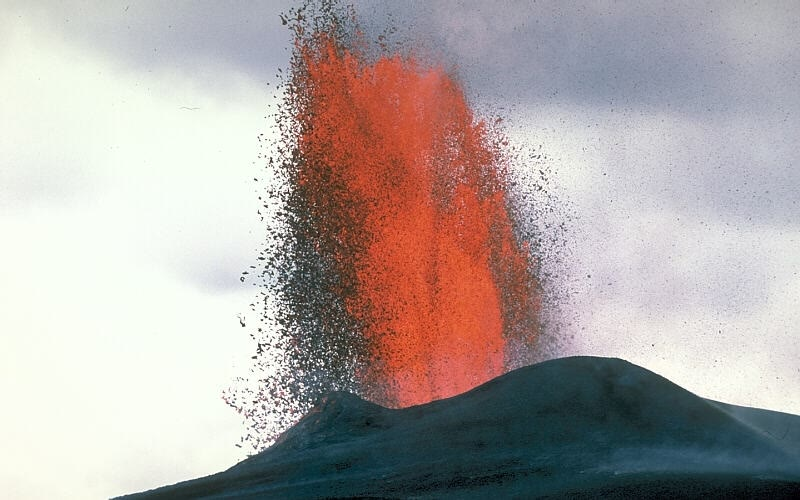
\includegraphics[height=4.3cm]{images/book4/b2-kilauea-fountain.jpg}\hfill
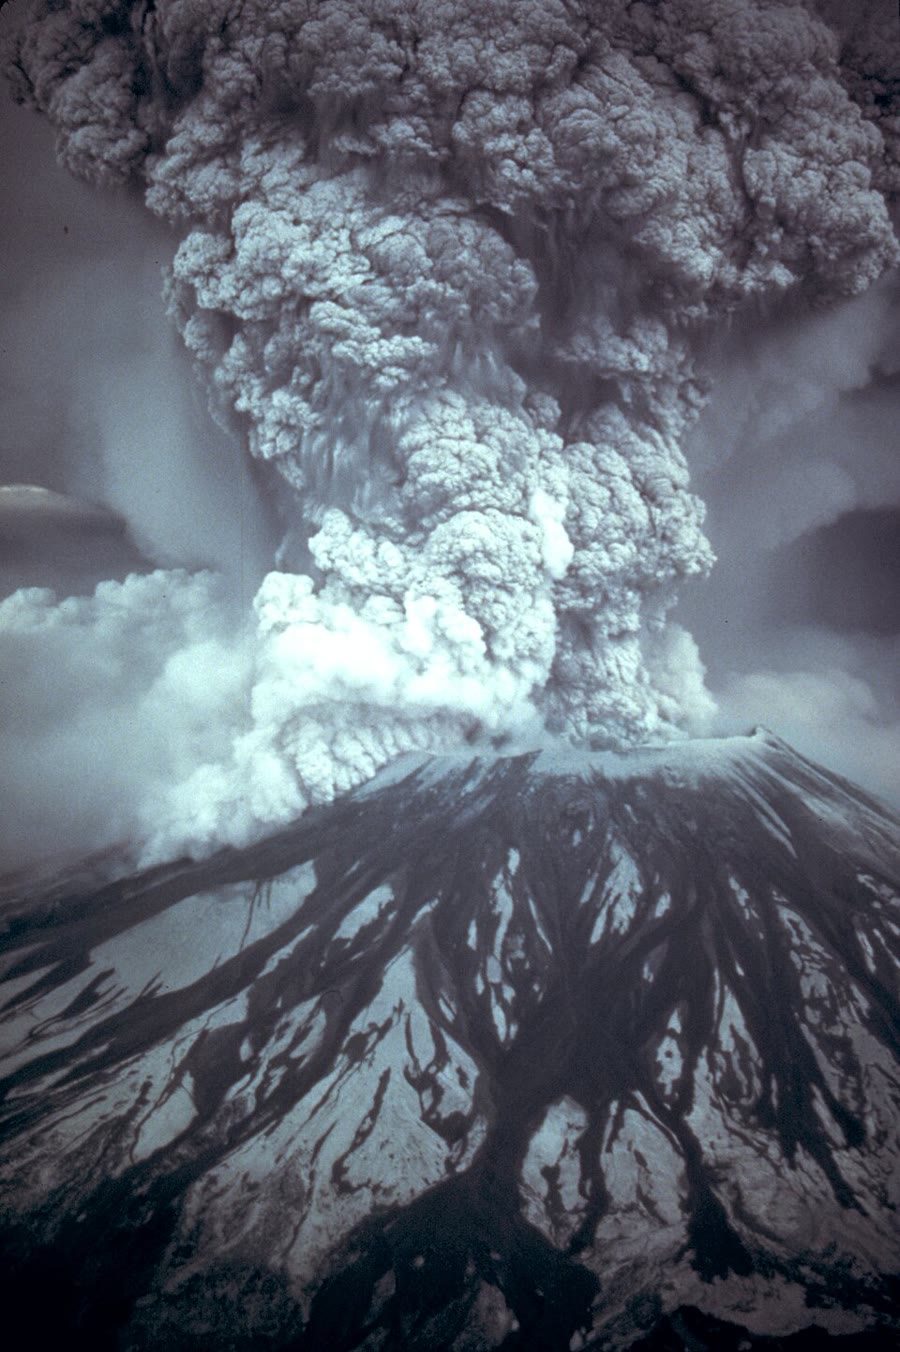
\includegraphics[height=4.3cm]{images/book4/b2-st-helens-column.jpg}\hfill
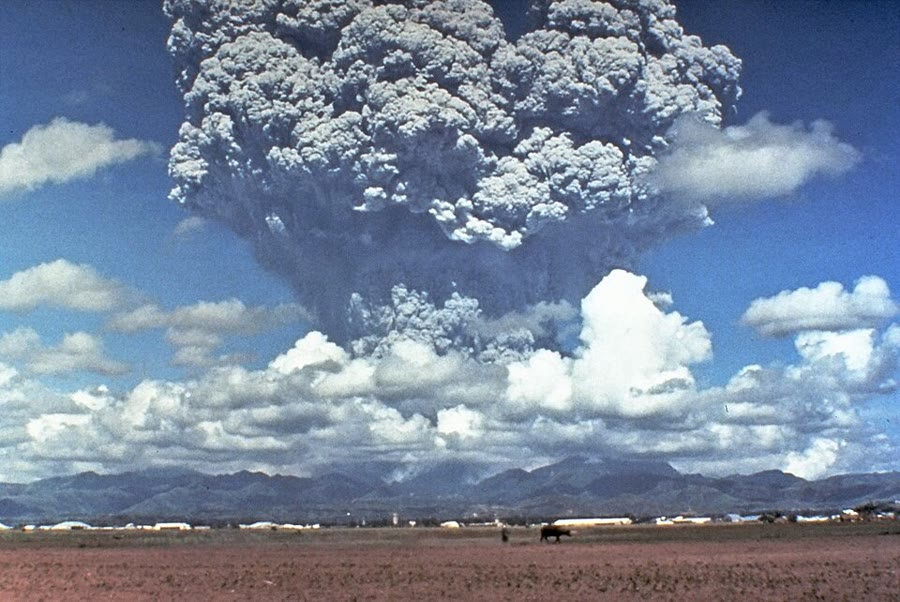
\includegraphics[height=4.3cm]{images/book4/b2-pinatubo-column.jpg}
\par\smallskip{\small Izquierda: una fuente hawaiana en el cono del Pu`u~`\=O`\=o, en el Kīlauea,
octubre de 1983 (J.\,D.~Griggs, USGS). Centro: la columna pliniana del monte Santa Helena,
18 de mayo de 1980 (Austin Post, USGS). Derecha: la \omterm{def:b2:eruptive-styles:column}{columna eruptiva} del monte Pinatubo el
12 de junio de 1991, tres días antes de la erupción paroxísmica (Dave Harlow, USGS). Las
tres fotografías son de dominio público.}
\end{omfigure}
% ledger: usgs:puuoo, usgs:msh-may18, usgs:pinatubo-1991

\section{Las columnas eruptivas}

\begin{definition}[Columna eruptiva]\label{def:b2:eruptive-styles:column}
Una \emph{columna eruptiva}\index{columna eruptiva} es la masa ascendente de gas y
fragmentos que se alza sobre una boca explosiva. Tiene tres partes: un \emph{chorro}, o
región de empuje del gas, en la que la mezcla sale de la boca deprisa pero más densa que el
aire y sube por su cantidad de movimiento; una región \emph{convectiva}, en la que la mezcla,
tras englobar y calentar aire suficiente para volverse más ligera que su entorno,
sube por flotabilidad; y una nube en \emph{paraguas}, que se extiende lateralmente al
nivel en el que la densidad de la columna iguala la de la atmósfera.
\end{definition}
% ledger: usgs:glossary-ch6, nps:styles, aubry23:fits

\begin{omfigure}
\centering
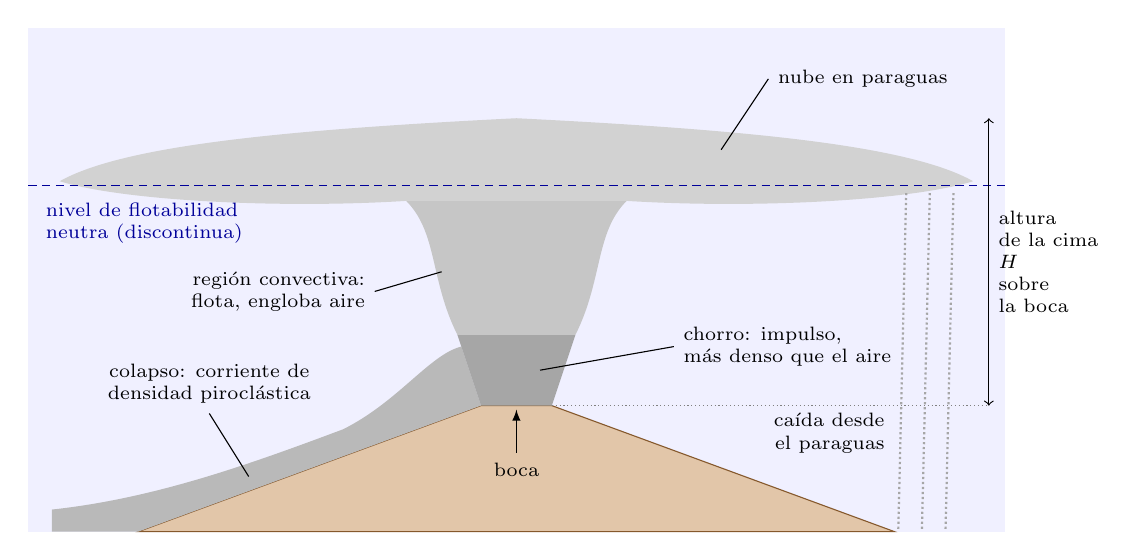
\begin{tikzpicture}[x=1cm, y=1cm, font=\scriptsize]
% atmosphere and ground
\fill[blue!6] (-6.2,0) rectangle (6.2,6.4);
% volcano
\fill[brown!45, draw=brown!70!black] (-4.8,0) -- (-0.45,1.6) -- (0.45,1.6) -- (4.8,0) -- cycle;
% collapse branch (left): a density current hugging the flank
\fill[gray!55] (-0.45,1.6) -- (-0.7,2.35) .. controls (-1.1,2.25) and (-1.5,1.65) .. (-2.2,1.3)
  .. controls (-3.4,0.85) and (-4.6,0.42) .. (-5.9,0.28) -- (-5.9,0) -- (-4.8,0) -- cycle;
% jet
\fill[gray!70] (-0.45,1.6) -- (0.45,1.6) -- (0.75,2.5) -- (-0.75,2.5) -- cycle;
% convective column
\fill[gray!45] (-0.75,2.5) .. controls (-1.1,3.2) and (-1.0,3.8) .. (-1.4,4.2)
  -- (1.4,4.2) .. controls (1.0,3.8) and (1.1,3.2) .. (0.75,2.5) -- cycle;
% umbrella
\fill[gray!35] (-1.4,4.2) .. controls (-3,4.1) and (-5,4.2) .. (-5.8,4.45)
  .. controls (-5,4.9) and (-3,5.1) .. (0,5.25) .. controls (3,5.1) and (5,4.9) .. (5.8,4.45)
  .. controls (5,4.2) and (3,4.1) .. (1.4,4.2) -- cycle;
\draw[densely dashed, blue!60!black] (-6.2,4.4) -- (6.2,4.4);
% fallout from the far end of the umbrella, down to the ground
\foreach \x in {4.95,5.25,5.55} {\draw[gray!70, densely dotted, thick] (\x,4.3) -- (\x-0.1,0.02);}
\draw[gray, densely dotted] (0.45,1.6) -- (6.0,1.6);
\draw[<->] (6.0,1.6) -- (6.0,5.25) node[midway, right, align=left] {altura\\de la cima\\$H$\\sobre\\la boca};
% labels
\node[anchor=north west, align=left, blue!60!black] at (-6.1,4.3) {nivel de flotabilidad\\neutra (discontinua)};
\draw (-0.95,3.3) -- (-1.8,3.05) node[left, align=right] {región convectiva:\\flota, engloba aire};
\draw (0.3,2.05) -- (2.0,2.35) node[right, align=left] {chorro: impulso,\\más denso que el aire};
\draw (2.6,4.85) -- (3.2,5.75) node[right] {nube en paraguas};
\node[anchor=east, align=right] at (4.8,1.25) {caída desde\\el paraguas};
\draw (-3.4,0.7) -- (-3.9,1.5) node[above, align=center] {colapso: corriente de\\densidad piroclástica};
\draw[-latex] (0,1.0) -- (0,1.55);
\node[anchor=north] at (0,1.0) {boca};
\end{tikzpicture}
\par\smallskip{\small Anatomía de una \omterm{def:b2:eruptive-styles:column}{columna eruptiva} (esquema, sin escala). A
la derecha la columna sube por sus tres regiones y la nube en paraguas
deja caer \omterm{def:b2:eruptive-styles:tephra}{tefra} al extenderse; a la izquierda, parte del chorro no ha logrado volverse
flotante y colapsa en una \omterm{def:b2:eruptive-styles:pdc}{corriente de densidad piroclástica}.}
\end{omfigure}

La altura que alcanza una columna depende ante todo del calor que aporta cada
segundo, es decir, del caudal másico eruptivo~$Q$. El análisis dimensional da la
forma de la ley.

\begin{proposition}[Altura de una pluma flotante]\label{prop:b2:eruptive-styles:plume}
Si la altura de la cima $H$ de una pluma flotante sobre una fuente puntual estacionaria depende solo
del flujo de flotabilidad $F$ de la fuente (de dimensión $\mathrm{m^4\,s^{-3}}$) y de la
frecuencia de flotabilidad $N$ de una atmósfera establemente estratificada (de dimensión
$\mathrm{s^{-1}}$), entonces
\[
H = c\,F^{1/4}N^{-3/4}
\]
con $c$ una constante adimensional. Como $F$ es proporcional al flujo de calor, y por tanto
al caudal másico eruptivo, $H \propto Q^{1/4}$ en una atmósfera dada.
\end{proposition}

\begin{proof}
Escríbase $H = c\,F^{\alpha}N^{\beta}$. Igualar las longitudes da $4\alpha = 1$; igualar
los tiempos da $-3\alpha - \beta = 0$. Por tanto $\alpha = 1/4$ y $\beta = -3/4$, y ninguna
otra combinación de $F$ y $N$ tiene la dimensión de una longitud.
\end{proof}

La constante $c$ procede de la rapidez con que la pluma engloba aire, que la teoría de plumas
trata con un coeficiente de arrastre medido en experimentos; aquí se
admite. Las columnas reales no son fuentes puntuales estacionarias en una atmósfera en calma, de modo que
los vulcanólogos ajustan la ley a erupciones cuya altura y cuyo caudal másico eruptivo se
midieron ambos.
% ledger: aubry23:fits

\begin{proposition}[Altura de la columna y caudal másico eruptivo]\label{prop:b2:eruptive-styles:mastin}
Con la altura de la cima $H$ sobre la boca en kilómetros y el caudal másico eruptivo
$Q$ en kilogramos por segundo, la compilación de erupciones bien documentadas da
\[
H = 0.304\,Q^{0.241},
\]
y un conjunto de datos mayor e independiente, de 130 sucesos, da $H = 0.345\,Q^{0.226}$.
La dispersión es grande: el error cuadrático medio relativo en $H$ es de un
\qtyrange{53}{60}{\percent}.
\end{proposition}
\admitted
% ledger: aubry23:fits

Ambos exponentes están cerca del $1/4$ de la teoría de plumas. La figura siguiente muestra
los dos ajustes y las erupciones de ejemplo en las que se basan los parámetros de fuente que usan
los centros de pronóstico de ceniza. Una columna de \qty{15}{km} de altura, como la del monte
Santa Helena, necesita \qty{e7}{kg/s}, diez mil toneladas cada segundo; duplicar la
altura requiere casi dieciocho veces ese caudal. Leída al revés, una altura medida da
el caudal, pero solo con un margen de un factor de varios, porque $Q$ va como $H^4$
(\cref{exo:b2:eruptive-styles:3}). Los vulcanólogos expresan el caudal mediante la \emph{intensidad} $I =
\log_{10}Q + 3$, con $Q$ en kilogramos por segundo.
% ledger: mastin09:examples, aubry23:fits, brown14:record

\begin{omfigure}
\centering
\begin{tikzpicture}
\begin{axis}[omrecord, width=0.82\linewidth, height=6cm, xmode=log, ymode=log,
  xmin=1e3, xmax=1e9, ymin=1, ymax=60,
  xlabel={caudal másico eruptivo $Q$ (\unit{kg/s})}, ylabel={altura de la cima sobre la boca (\unit{km})},
  ytick={1,2,5,10,20,50}, yticklabels={1,2,5,10,20,50},
  legend pos=north west, legend style={font=\scriptsize},
  tick label style={font=\scriptsize}, label style={font=\small}]
\addplot[very thick, black] table[x=Q, y=mastin] {figdata/out/bachelor-2-eruptions-column.dat};
\addlegendentry{$H = 0.304\,Q^{0.241}$}
\addplot[thick, red!70!black, dashed] table[x=Q, y=aubry] {figdata/out/bachelor-2-eruptions-column.dat};
\addlegendentry{$H = 0.345\,Q^{0.226}$}
\addplot[only marks, mark=*, mark size=1.8pt, blue!70!black]
  table[x=Q, y=H] {figdata/out/bachelor-2-eruptions-column-data.dat};
\addlegendentry{erupciones de ejemplo}
\begin{scope}[font=\tiny, inner sep=1.5pt]
\node[anchor=north west] at (axis cs:5e3,2) {Etna 2001};
\node[anchor=south east] at (axis cs:1e5,7) {Cerro Negro 1992};
\node[anchor=north west] at (axis cs:2e5,5) {Ruapehu 1996};
\node[anchor=east] at (axis cs:1e6,10) {Fuego 1974};
\draw[gray] (axis cs:3e6,10) -- (axis cs:2e7,4.5) node[anchor=west, black] {Soufrière Hills};
\draw[gray] (axis cs:4e6,11) -- (axis cs:2e7,6.5) node[anchor=west, black] {Spurr 1992};
\node[anchor=south east] at (axis cs:1e7,15) {St Helens 1980};
\node[anchor=south east, align=right] at (axis cs:1e8,25) {St Helens\\coignimbrítica};
\end{scope}
\end{axis}
\end{tikzpicture}
\par\smallskip{\small Altura de la cima de las \omterm{def:b2:eruptive-styles:column}{columnas eruptivas} sobre la boca frente al
caudal másico eruptivo: el ajuste empírico de Mastin y colaboradores (2009), el ajuste de
Aubry y colaboradores (2023) a un conjunto de datos independiente, y las erupciones de ejemplo
de la primera compilación (la nube coignimbrítica del monte Santa Helena subió desde
\omterm{def:b2:eruptive-styles:pdc}{flujos piroclásticos}, no desde la boca).}
\end{omfigure}
% ledger: aubry23:fits, mastin09:examples

Una columna también puede no lograr subir. El chorro sale de la boca más denso que el aire; si
se queda sin cantidad de movimiento antes de haber englobado aire suficiente para volverse flotante,
por ejemplo porque baja su contenido en gas, la columna colapsa y la mezcla
desciende por los flancos como una corriente caliente y densa. Las columnas plinianas pueden colapsar de
este modo, y en el Pinatubo los \omterm{def:b2:eruptive-styles:pdc}{flujos piroclásticos} de 1991 rellenaron valles con
depósitos de hasta \qty{200}{m} de espesor.
% ledger: nps:styles, usgs:pinatubo-deposits

\section{Los productos piroclásticos}

\begin{definition}[Tefra y piroclastos]\label{def:b2:eruptive-styles:tephra}
Un \emph{piroclasto}\index{piroclasto} es un fragmento producido por la fragmentación
explosiva del \omterm{def:b2:magma-emplacement:magma}{magma} o de las rocas que lo rodean. La \emph{tefra}\index{tefra} es
el nombre colectivo de todos los piroclastos lanzados al aire, sea cual sea su tamaño.
Por tamaño, los piroclastos de menos de \qty{2}{mm} forman la ceniza volcánica; los de
\qtyrange{2}{64}{mm} son \emph{lapilli}\index{lapilli}; los de más de
\qty{64}{mm} son bloques si eran sólidos al ser expulsados y son angulosos, y una
\emph{bomba volcánica}\index{bomba volcánica} si estaban total o parcialmente fundidos
y tomaron en vuelo una forma redondeada o de huso.
\end{definition}
% ledger: nps:pyroclast-sizes, usgs:glossary-ch6

La \omterm{def:b2:eruptive-styles:tephra}{tefra} cae de la nube en paraguas y de la columna, a sotavento, como un depósito de caída
que cubre el terreno: grueso cerca de la boca, más delgado y fino lejos de ella. Su
espesor se cartografía mediante \emph{isópacas}, líneas de igual espesor, y, por regla general,
decrece exponencialmente con la distancia. Como el viento estira las isópacas
en elipses, la distancia se mide mejor por la raíz cuadrada del área que encierra cada
isópaca.
% ledger: usgs:ash-props, biass19:layer5

\begin{proposition}[Volumen de un depósito que se adelgaza exponencialmente]\label{prop:b2:eruptive-styles:thinning}
Si el espesor de un depósito de caída decrece con la raíz cuadrada $x = \sqrt A$
del área de la isópaca como $T = T_0\,e^{-kx}$, su volumen aparente es
\[
V = \frac{2T_0}{k^2}.
\]
La mitad de ese volumen queda más allá de la isópaca $x_{1/2} = 1.678/k$.
\end{proposition}

\begin{proof}
Entre las isópacas de áreas $A$ y $A + dA$ el depósito tiene un volumen $T\,dA$,
y $dA = 2x\,dx$. Así, $V = \int_0^\infty T_0e^{-kx}\,2x\,dx = 2T_0/k^2$, por
integración por partes ($\int_0^\infty xe^{-kx}dx = 1/k^2$). El volumen dentro de $x$
es $\frac{2T_0}{k^2}[1 - (1 + kx)e^{-kx}]$, que es la mitad del total cuando $(1 +
u)e^{-u} = 1/2$ con $u = kx$, es decir, $u = 1.678$.
\end{proof}

Los depósitos reales se adelgazan con dos o más pendientes, fuerte cerca de la boca y suave lejos,
porque los \omterm{def:b2:eruptive-styles:tephra}{lapilli} gruesos caen deprisa de la columna y la ceniza fina
deriva. Cada segmento se ajusta por separado y la integral se calcula por
tramos.

\begin{method}[Volumen de un depósito de caída a partir de sus isópacas]\label{met:b2:eruptive-styles:volume}
Represéntese $\ln T$ frente a $\sqrt A$ para cada isópaca y ajústese una recta a cada
serie de puntos alineados. Para dos segmentos, $T_0e^{-k_1x}$ dentro del punto de corte
$X$ de las dos rectas y el segundo más allá, el volumen es
\[
V = \frac{2T_0}{k_1^2} + 2T_0e^{-k_1X}\left[\frac{k_2X + 1}{k_2^2} -
\frac{k_1X + 1}{k_1^2}\right]
\]
(\cref{exo:b2:eruptive-styles:10}). El volumen aparente se convierte en un equivalente en roca densa, el volumen de
la misma masa como \omterm{def:b2:magma-emplacement:magma}{magma} sin burbujas, mediante $V_{\mathrm{DRE}} = V\rho_{\mathrm{deposit}}/\rho_{\mathrm{magma}}$.
\end{method}
% ledger: biass19:layer5, brown14:record

La figura siguiente aplica el método a una caída de escorias emitida por el Cotopaxi, en
Ecuador, hace unos \num{1200} años. Dos segmentos se ajustan a las seis isópacas, con
distancias de reducción del espesor a la mitad, $\ln 2/k$, de \qty{1.9}{km} y \qty{5.0}{km} (el
estudio publicado, cuyo ajuste difiere ligeramente, halla \qty{1.9}{km} y
\qty{5.3}{km}), y el volumen resulta de \qty{0.29}{km^3}, como en ese estudio. Más del
\qty{40}{\percent} de él está en el delgado segmento distal, y por eso la ceniza distal,
fácilmente erosionada o nunca cartografiada, pesa tanto en el total. La ceniza recién caída
tiene una densidad aparente de \qtyrange{500}{1500}{kg/m^3}, muy por debajo de la del
\omterm{def:b2:magma-emplacement:magma}{magma}, de modo que el equivalente en roca densa es aproximadamente la mitad del volumen aparente o menos.
% ledger: biass19:layer5, usgs:ash-props

\begin{omfigure}
\centering
\begin{tikzpicture}
\begin{axis}[omrecord, width=0.78\linewidth, height=5.6cm, ymode=log,
  xmin=0, xmax=30, ymin=2, ymax=2000,
  xlabel={$\sqrt{\text{área de la isópaca}}$ (\unit{km})}, ylabel={espesor (\unit{cm})},
  ytick={2,5,10,20,50,100,200,500,1000,2000}, yticklabels={2,5,10,20,50,100,200,500,1000,2000},
  legend pos=north east, legend style={font=\scriptsize},
  tick label style={font=\scriptsize}, label style={font=\small}]
\addplot[thick, black, restrict x to domain=0:12] table[x=sqrtA_km, y=seg1] {figdata/out/bachelor-2-eruptions-thin-fit.dat};
\addlegendentry{segmento proximal, $k_1 = \qty{0.365}{km^{-1}}$}
\addplot[thick, red!70!black, dashed, restrict x to domain=5:30] table[x=sqrtA_km, y=seg2] {figdata/out/bachelor-2-eruptions-thin-fit.dat};
\addlegendentry{segmento distal, $k_2 = \qty{0.138}{km^{-1}}$}
\addplot[only marks, mark=*, mark size=2pt, blue!70!black] table[x=sqrtA_km, y=T_cm] {figdata/out/bachelor-2-eruptions-thin-data.dat};
\addlegendentry{isópacas}
\end{axis}
\end{tikzpicture}
\par\smallskip{\small Adelgazamiento de la caída de escorias de la capa~5 del Cotopaxi (Ecuador),
de unos \num{1200} años de antigüedad: espesores de las isópacas según Biass, Bonadonna y
Houghton (2019) frente a la raíz cuadrada del área que encierra cada isópaca (la
escala vertical es logarítmica). Dos segmentos exponenciales, ajustados a las dos
isópacas proximales y a las cuatro distales, se cortan en $\sqrt A = \qty{8.6}{km}$;
integrados, dan un volumen aparente de \qty{0.29}{km^3}.}
\end{omfigure}
% ledger: biass19:layer5

No toda la \omterm{def:b2:eruptive-styles:tephra}{tefra} cae del cielo. Cuando una columna colapsa, un domo se desmorona o una
explosión lateral abre el flanco de un volcán, la mezcla caliente corre a ras de
suelo.

\begin{definition}[Corrientes de densidad piroclástica]\label{def:b2:eruptive-styles:pdc}
Una \emph{corriente de densidad piroclástica}\index{corriente de densidad piroclástica} es una
mezcla de gas caliente y \omterm{def:b2:eruptive-styles:tephra}{piroclastos} pegada al suelo que fluye pendiente abajo o hacia fuera
porque es más densa que el aire. Un \emph{flujo piroclástico}\index{flujo piroclástico}
es una corriente concentrada de fragmentos de roca, ceniza y gas, en general de
\qtyrange{200}{700}{\celsius}, que se desplaza a decenas de metros por segundo; una
\emph{oleada piroclástica}\index{oleada piroclástica} es una nube más diluida de ceniza,
roca y gas, de varios cientos de grados, que se desplaza a la velocidad de un viento
huracanado. Una \emph{ignimbrita}\index{ignimbrita} es la roca depositada por las corrientes de
densidad piroclástica, que puede quedar soldada por su propio calor.
\end{definition}
% ledger: usgs:glossary-ch6

El 18 de mayo de 1980 el colapso del flanco norte del monte Santa Helena, el mayor
deslizamiento de la historia registrada, con unos \qty{2.8}{km^3}, destechó el \omterm{def:b2:magma-emplacement:magma}{magma} y
liberó una explosión lateral que barrió unos \qty{600}{km^2} a velocidades de hasta
\qty{480}{km/h}; \omterm{def:b2:eruptive-styles:pdc}{flujos piroclásticos} de al menos \qty{700}{\celsius} llegaron después a
\qty{8}{km} del cráter. Los flujos de 1991 del Pinatubo seguían a
\qty{500}{\celsius} en su interior cinco años después.
% ledger: usgs:msh-may18, usgs:msh-flows, usgs:msh-reach, usgs:pinatubo-deposits

\begin{definition}[Lahar]\label{def:b2:eruptive-styles:lahar}
Un \emph{lahar}\index{lahar} es una mezcla rápida de agua y derrubios volcánicos
que desciende por un valle fluvial, con una consistencia que va del agua fangosa
al hormigón húmedo. Los lahares se forman cuando las corrientes piroclásticas funden la nieve y el hielo, cuando
caen lluvias intensas sobre depósitos volcánicos sueltos, cuando se rompe un lago represado por depósitos
volcánicos, o a partir de una avalancha de derrubios.
\end{definition}
% ledger: usgs:glossary-ch6

Los \omterm{def:b2:eruptive-styles:lahar}{lahares} sobreviven a las erupciones. Alrededor del Pinatubo, las lluvias del monzón y de los tifones convirtieron la
ceniza de 1991 en \omterm{def:b2:eruptive-styles:lahar}{lahares} durante años, y causaron más destrucción que la
propia erupción.
% ledger: usgs:pinatubo-lahars

\begin{definition}[Caldera]\label{def:b2:eruptive-styles:caldera}
Una \emph{caldera}\index{caldera} es una gran depresión volcánica en forma de cuenca,
de \qtyrange{2}{50}{km} de diámetro y mucho más ancha que cualquier boca de su interior, formada por
el hundimiento del terreno en un reservorio magmático somero que una erupción ha
vaciado en parte.
\end{definition}
% ledger: usgs:glossary-ch6

Las \omterm{def:b2:eruptive-styles:caldera}{calderas} del Pinatubo y del Novarupta miden ambas unos \qty{2.5}{km} de diámetro, en el
extremo inferior de la gama. Una \omterm{def:b2:eruptive-styles:caldera}{caldera} se distingue de un cráter, que es menor y está excavado por explosiones.
% ledger: usgs:pinatubo-1991, nps:styles, usgs:glossary-ch6

\section{Medir y contar las erupciones}

\begin{definition}[Índice de explosividad volcánica]\label{def:b2:eruptive-styles:vei}
El \emph{índice de explosividad volcánica}\index{indice de explosividad volcánica@índice de explosividad volcánica} (VEI) es
un entero de 0 a 8 que mide el tamaño de una erupción, sobre todo por el
volumen aparente de su \omterm{def:b2:eruptive-styles:tephra}{tefra}: VEI~0 para menos de \qty{e4}{m^3}, VEI~1 hasta
\qty{e6}{m^3}, y luego un escalón por cada factor diez, hasta VEI~8 por encima de
\qty{e12}{m^3}, \qty{1000}{km^3}. La altura de la columna y las descripciones de la erupción
se usan cuando no se conoce el volumen. Una erupción no explosiva tiene VEI~0,
sea cual sea el volumen de su lava.
\end{definition}
% ledger: usgs:vei-criteria, usgs:msh-comparisons

\begin{table}[ht]
\centering
\small
\begin{tabular}{llll}
\hline
VEI & volumen aparente de \omterm{def:b2:eruptive-styles:tephra}{tefra} (\unit{m^3}) & altura de la columna (\unit{km}) & estilo habitual \\
\hline
0 & $< 10^{4}$ & $< 0.1$ & hawaiano \\
1 & $10^{4}$--$10^{6}$ & 0.1--1 & hawaiano, estromboliano \\
2 & $10^{6}$--$10^{7}$ & 1--5 & estromboliano, vulcaniano \\
3 & $10^{7}$--$10^{8}$ & 3--15 & vulcaniano \\
4 & $10^{8}$--$10^{9}$ & 10--25 & vulcaniano, pliniano \\
5 & $10^{9}$--$10^{10}$ & $> 25$ & pliniano \\
6 & $10^{10}$--$10^{11}$ & $> 25$ & pliniano \\
7 & $10^{11}$--$10^{12}$ & $> 25$ & pliniano \\
8 & $> 10^{12}$ & $> 25$ & pliniano \\
\hline
\end{tabular}
\caption{Criterios del \omterm{def:b2:eruptive-styles:vei}{índice de explosividad volcánica} (según Newhall y Self, 1982).}
\label{tab:b2:eruptive-styles:vei}
\end{table}
% ledger: usgs:vei-criteria

El índice es logarítmico como una magnitud sísmica, pero más grueso. El monte
Santa Helena en 1980, con \qty{1.3}{km^3} de ceniza, recibió un VEI~5 «por los pelos»;
el Pinatubo en 1991, un VEI~6; el Tambora en 1815, que expulsó de treinta a ochenta
veces más ceniza que el monte Santa Helena, un VEI~7, la mayor \omterm{def:b2:eruptive-styles:regimes}{erupción explosiva}
de los tiempos históricos. Para el trabajo cuantitativo los vulcanólogos prefieren la
\emph{magnitud} $M = \log_{10}m - 7$, con $m$ la masa emitida en kilogramos, que
evita la densidad aparente del depósito, y la intensidad definida más arriba para el
caudal.
% ledger: usgs:msh-1980-ash, usgs:msh-comparisons, data:b4-gvp-eruptions, brown14:record

Las erupciones pequeñas son frecuentes y las grandes, raras. El catálogo mundial de
erupciones del Holoceno hace cuantitativa la relación, una vez que se tienen en cuenta sus
lagunas: una erupción solo figura en el catálogo si alguien la registró o encontró su
depósito, y las erupciones pequeñas lejos de los observadores, o de más de unos pocos siglos de
antigüedad, a menudo se pasaron por alto. El registro de las grandes erupciones es completo durante más tiempo que
el de las pequeñas. En el panel izquierdo de la figura siguiente, las erupciones de cada
tamaño registradas desde 1500 se acumulan con el tiempo; un registro completo a ritmo
constante seguiría la diagonal. Las erupciones de VEI~3 o más se agolpan en el último
siglo, porque la mayoría de las anteriores nunca se registraron; el registro de VEI~6
está cerca de la diagonal.
% ledger: data:b4-gvp-eruptions, brown14:record

\begin{dated}{2026}
El catálogo del Global Volcanism Program recoge \num{7747} erupciones holocenas confirmadas
con un VEI. Contando desde el inicio de una ventana hasta el final de 2024, hubo
399 erupciones de VEI~3 o más desde 1950, 95 de VEI~4 o más desde 1900,
22 de VEI~5 o más desde 1800 y 8 de VEI~6 o más desde 1500 (la más
reciente, el Pinatubo en 1991). Solo se registran dos erupciones de VEI~7 desde el año
1000: el Rinjani en 1257 y el Tambora, cuya erupción empezó en 1812 y culminó en
1815.
\end{dated}
% ledger: data:b4-gvp-eruptions, usgs:msh-comparisons

\begin{proposition}[Ley frecuencia--tamaño de las erupciones]\label{prop:b2:eruptive-styles:frequency}
Sea $\lambda_v$ el número medio de erupciones de VEI $\ge v$ por año en la Tierra,
estimado cada uno en una ventana en la que su registro es casi completo (desde 1950
para $v = 3$, 1900 para $v = 4$, 1800 para $v = 5$, 1500 para $v = 6$). Entonces, por mínimos
cuadrados,
\[
\log_{10}\lambda_v = 3.28 - 0.85\,v .
\]
Cada escalón de VEI es unas siete veces más raro que el anterior.
\end{proposition}
% ledger: data:b4-gvp-eruptions

La ley es empírica, un ajuste a cuatro puntos, y su exponente depende de las
ventanas elegidas; predice una erupción de VEI~7 o más cada \num{470} años,
cerca de las dos de los últimos mil años, que no se usaron para ajustarla. Como
las erupciones son casi independientes entre sí, se comportan como un proceso
de Poisson, y la probabilidad de al menos una erupción de VEI $\ge v$ en $t$ años
es $1 - e^{-\lambda_vt}$ (problema de fin de semana).
% ledger: data:b4-gvp-eruptions

\begin{omfigure}
\centering
\begin{tikzpicture}
\begin{axis}[omrecord, name=cum, width=0.47\linewidth, height=5.6cm,
  xmin=1500, xmax=2024, ymin=0, ymax=1,
  xlabel={año}, ylabel={fracción registrada desde 1500},
  xtick={1500,1600,1700,1800,1900,2000}, x tick label style={/pgf/number format/1000 sep={}},
  legend pos=north west, legend style={font=\tiny},
  tick label style={font=\scriptsize}, label style={font=\small}]
\addplot[thick, gray, densely dotted, domain=1500:2024, samples=2] {(x - 1500)/524};
\addlegendentry{ritmo constante}
\addplot[thick, blue!70!black] table[x=year, y=f3] {figdata/out/bachelor-2-eruptions-vei-cumul.dat};
\addlegendentry{VEI $\ge 3$}
\addplot[thick, black, dashed] table[x=year, y=f4] {figdata/out/bachelor-2-eruptions-vei-cumul.dat};
\addlegendentry{VEI $\ge 4$}
\addplot[thick, orange!80!black, dashdotted] table[x=year, y=f5] {figdata/out/bachelor-2-eruptions-vei-cumul.dat};
\addlegendentry{VEI $\ge 5$}
\addplot[thick, red!70!black, const plot] table[x=year, y=f6] {figdata/out/bachelor-2-eruptions-vei-cumul.dat};
\addlegendentry{VEI $\ge 6$}
\end{axis}
\begin{axis}[omrecord, at={(cum.east)}, anchor=west, xshift=1.9cm,
  width=0.47\linewidth, height=5.6cm, ymode=log,
  xmin=2.5, xmax=7.5, ymin=1e-3, ymax=20,
  xlabel={VEI $v$}, ylabel={erupciones de VEI $\ge v$ por año},
  xtick={3,4,5,6,7},
  tick label style={font=\scriptsize}, label style={font=\small}]
\addplot[thick, black] table[x=vei, y=rate] {figdata/out/bachelor-2-eruptions-vei-fit.dat};
\addplot[only marks, mark=*, mark size=2pt, blue!70!black] table[x=vei, y=rate] {figdata/out/bachelor-2-eruptions-vei-rate.dat};
\addplot[only marks, mark=o, mark size=2.4pt, red!70!black] table[x=vei, y=rate] {figdata/out/bachelor-2-eruptions-vei-rate7.dat};
\node[font=\tiny, anchor=south west] at (axis cs:3.05,6) {desde 1950};
\node[font=\tiny, anchor=south west] at (axis cs:4.05,0.8) {desde 1900};
\node[font=\tiny, anchor=south west] at (axis cs:5.05,0.1) {desde 1800};
\node[font=\tiny, anchor=south west] at (axis cs:6.05,0.016) {desde 1500};
\node[font=\tiny, anchor=east, red!70!black] at (axis cs:6.85,0.00195) {desde 1000};
\end{axis}
\end{tikzpicture}
\par\smallskip{\small Izquierda: completitud del registro mundial. Para cada tamaño,
la fracción de las erupciones registradas entre 1500 y 2024 que ya se habían
producido en un año dado; un registro completo a ritmo constante seguiría la
diagonal de puntos. Derecha: ritmo anual de erupciones de VEI $\ge v$, cada una contada en
su propia ventana, y la recta de mínimos cuadrados de la
\cref{prop:b2:eruptive-styles:frequency}; el círculo vacío, VEI $\ge 7$ desde el año
1000, no se usó en el ajuste. Datos: Global Volcanism Program, Volcanoes of the
World.}
\end{omfigure}
% ledger: data:b4-gvp-eruptions

\section{Vigilar los volcanes}

El \omterm{def:b2:magma-emplacement:magma}{magma} no llega a la superficie sin avisar. Debe romper la roca para abrirse
camino, empuja el terreno hacia arriba a medida que se acumula, libera gas a medida que baja la presión
que soporta, y calienta el terreno. Los observatorios volcanológicos vigilan las cuatro cosas.

\emph{Sismicidad.} El \omterm{def:b2:magma-emplacement:magma}{magma} que se mueve por la corteza rompe la roca y desencadena enjambres
de pequeños terremotos. Antes del 18 de mayo de 1980 el monte Santa Helena produjo más de
\num{10000} en dos meses; el Pinatubo produjo miles entre abril y
junio de 1991, por un \omterm{def:b2:magma-emplacement:magma}{magma} que subía desde más de \qty{32}{km} de profundidad. Las magnitudes
y los momentos sísmicos del volumen de primer año se aplican sin cambios; lo que difiere son las
fuentes: grietas que se abren y conductos llenos de fluido que resuenan, además de las fallas.
% ledger: usgs:msh-lead-up, usgs:pinatubo-deposits

\emph{Deformación.} Un reservorio que se llena se hincha y levanta el terreno que tiene
encima. La nivelación, los inclinómetros y el posicionamiento por satélite miden el levantamiento; la interferometría radar desde satélite lo cartografía sobre volcanes
enteros, una técnica que explica el volumen de tercer año de esta serie. El modelo más
sencillo trata el reservorio como una pequeña esfera.

\begin{proposition}[Fuente de Mogi]\label{prop:b2:eruptive-styles:mogi}
Una pequeña fuente esférica a la profundidad $z_0$ en un semiespacio elástico homogéneo
con coeficiente de Poisson $\nu$, cuyo volumen cambia en $\Delta V$, una
\emph{fuente de Mogi}\index{fuente de Mogi}, levanta la superficie a la distancia horizontal $r$
en
\[
u_z(r) = \frac{(1 - \nu)\,\Delta V}{\pi}\,\frac{z_0}{(r^2 + z_0^2)^{3/2}} .
\]
\end{proposition}
\admitted
% ledger: dmodels:mogi

El levantamiento es máximo sobre la fuente, $u_z(0) = (1 - \nu)\Delta V/(\pi z_0^2)$, y
cae a la mitad en $r = z_0\sqrt{2^{2/3} - 1} = 0.766\,z_0$: la anchura del
abombamiento da la profundidad de la fuente, y su altura da entonces el cambio de
volumen. Como solo interviene $\Delta V$, la presión en el reservorio y su tamaño
no pueden separarse, de modo que lo que publican los geodestas son cambios de volumen, no presiones.
La fórmula es el primer término de una solución exacta para una esfera de radio
$a$; la corrección es del \qty{12}{\percent} cuando $a = z_0/2$ y del \qty{3}{\percent}
cuando $a = z_0/3$.
% ledger: dmodels:mogi

\begin{omfigure}
\centering
\begin{tikzpicture}
\begin{axis}[omrecord, width=0.78\linewidth, height=5.2cm,
  xmin=-12, xmax=12, ymin=0, ymax=65,
  xlabel={distancia horizontal a la fuente (\unit{km})}, ylabel={levantamiento (\unit{mm})},
  legend pos=north east, legend style={font=\scriptsize},
  tick label style={font=\scriptsize}, label style={font=\small}]
\addplot[very thick, black] table[x=r_km, y=z2] {figdata/out/bachelor-2-eruptions-mogi.dat};
\addlegendentry{fuente a \qty{2}{km}}
\addplot[very thick, red!70!black, dashed] table[x=r_km, y=z4] {figdata/out/bachelor-2-eruptions-mogi.dat};
\addlegendentry{fuente a \qty{4}{km}}
\draw[<->, thin] (axis cs:-1.532,29.8) -- (axis cs:1.532,29.8) node[midway, below, font=\tiny] {$2\times 0.766\,z_0$};
\end{axis}
\end{tikzpicture}
\par\smallskip{\small Levantamiento de la superficie sobre una \omterm{prop:b2:eruptive-styles:mogi}{fuente de Mogi} cuyo volumen crece en
\qty{e6}{m^3} ($\nu = 0.25$), a dos profundidades. Al doble de profundidad, el abombamiento es cuatro
veces más bajo y dos veces más ancho; la flecha marca la anchura total a media altura
del más somero.}
\end{omfigure}
% ledger: dmodels:mogi

\emph{Gas y calor.} A medida que el \omterm{def:b2:magma-emplacement:magma}{magma} sube y se desgasifica, el flujo de dióxido de azufre en la
superficie aumenta, y se mide desde el suelo, desde aviones y desde
satélites; el Pinatubo emitió muchos miles de toneladas en las semanas anteriores a su erupción.
El calor del \omterm{def:b2:magma-emplacement:magma}{magma} somero se ve en las imágenes térmicas del terreno y de la boca.
% ledger: usgs:pinatubo-deposits

A partir de estos datos un observatorio fija un nivel de alerta. En Estados Unidos, el
nivel de alerta volcánica en tierra (Volcano Alert Level), en uso desde 2006, tiene cuatro escalones, NORMAL,
ADVISORY, WATCH y WARNING, y un código de colores paralelo para la aviación, de GREEN a RED,
advierte a los aviones de la ceniza. No hay umbrales fijos: cada cambio lo deciden
los científicos del observatorio a partir de todos los datos de vigilancia, del comportamiento pasado
del volcán y de lo que se sabe de los procesos en curso. El pronóstico sigue siendo
probabilístico: cuándo empezará una erupción y cuál será su tamaño es difícil de
prever. En el Pinatubo, el pronóstico de 1991 permitió que la población que vivía cerca del
volcán se alejara a tiempo y salvó al menos \num{5000} vidas. Cómo entran esos pronósticos
en las decisiones sobre peligro y riesgo corresponde al \cref{ch:b2:geological-hazards}.
% ledger: hvo:alert-levels, usgs:pinatubo-1991

\begin{inthefield}[En un observatorio volcanológico]
\begin{minipage}[t]{0.6\linewidth}\vspace{0pt}
Un observatorio vigila sus volcanes día y noche. Los sismómetros de los flancos
envían sus señales por radio a pantallas en las que los científicos de guardia buscan enjambres,
tremor, la vibración continua del fluido que se mueve en un conducto, y cambios
en la profundidad de los sucesos. Las estaciones de posicionamiento y los inclinómetros registran la
hinchazón del terreno, las cámaras la boca, los espectrómetros de gas el flujo de dióxido
de azufre en la pluma. Cuando una señal se aparta del fondo habitual del volcán, los
científicos la comparan con episodios anteriores, se reúnen y deciden si el nivel de alerta
debe cambiar; el aviso que publican indica lo que se observa y lo que puede
seguir, sin exagerar ni lo uno ni lo otro.
\end{minipage}\hfill
\begin{minipage}[t]{0.36\linewidth}\vspace{0pt}
\centering
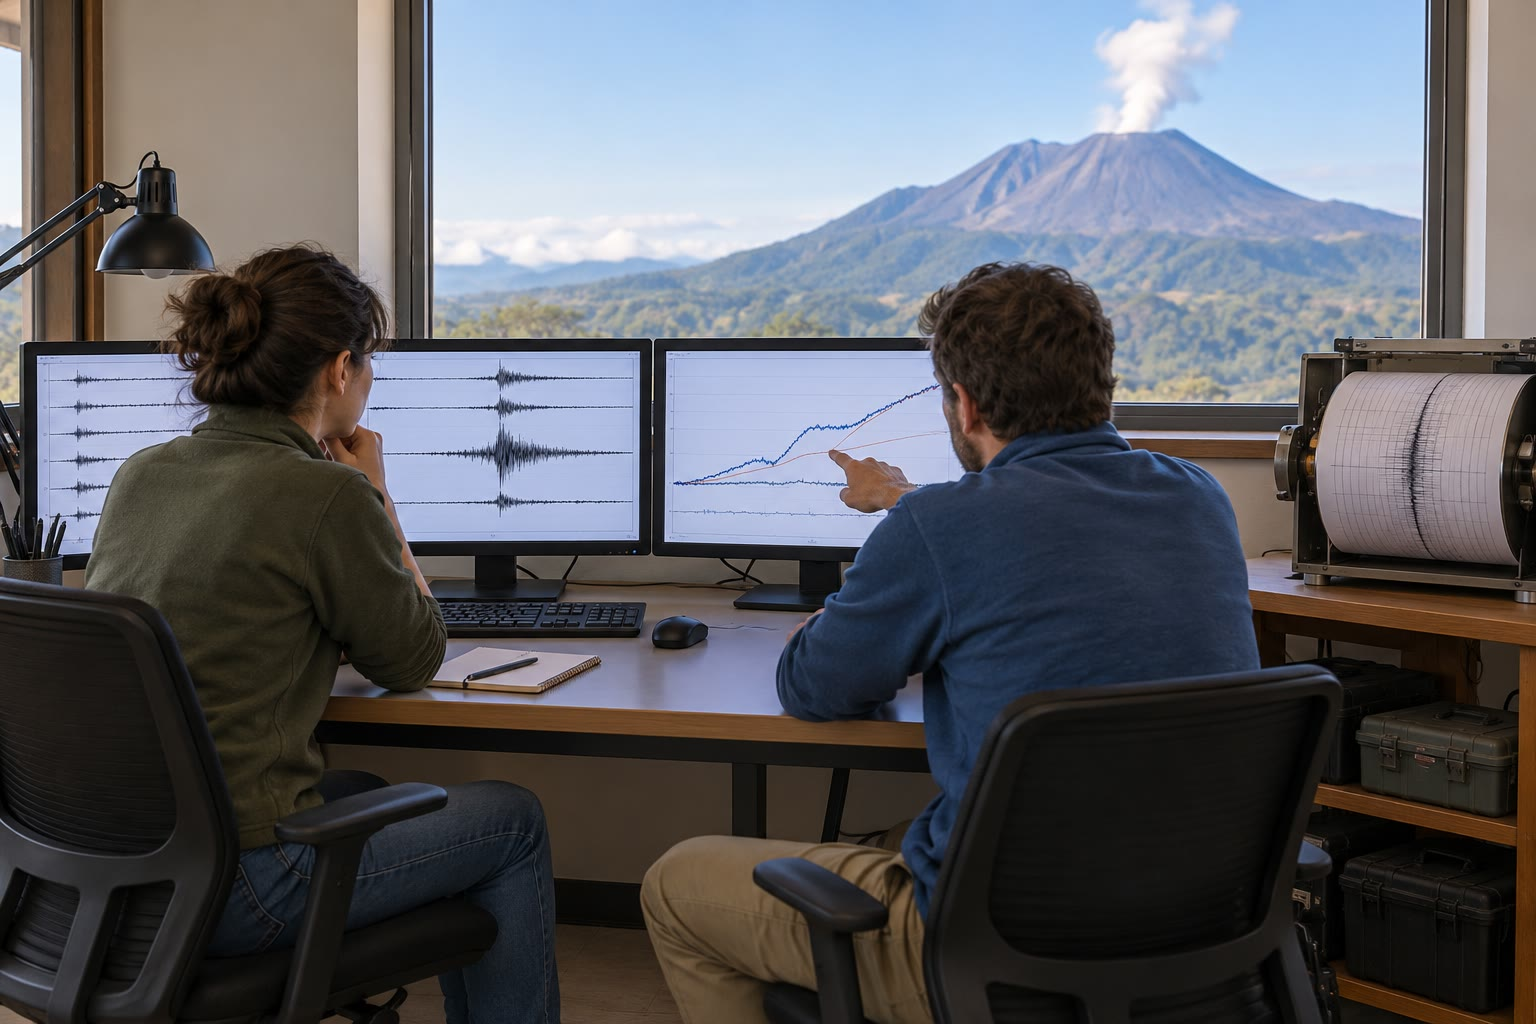
\includegraphics[width=\linewidth]{images/book4/ai/b2-volcano-observatory.jpg}
\par\smallskip{\scriptsize Científicos revisando registros sísmicos en un observatorio
volcanológico (ilustración generada por IA).}
\end{minipage}
\end{inthefield}
% ledger: hvo:alert-levels

\section{Ejercicios}

\begin{exercise}[$\star$]\label{exo:b2:eruptive-styles:1}
Dese el VEI que indica el solo volumen aparente de \omterm{def:b2:eruptive-styles:tephra}{tefra} para: (a) la ceniza del
monte Santa Helena, 18 de mayo de 1980, \qty{1.3}{km^3}; (b) la caída de la capa~5 del Cotopaxi,
\qty{0.29}{km^3}; (c) una pequeña erupción de \qty{2e6}{m^3}. (d) El material
expulsado por el Pinatubo en 1991 se da como «más de \qty{5}{km^3}», y sin embargo la
erupción tiene un VEI~6. ¿Qué volumen aparente implica como mínimo esa clasificación?
\end{exercise}
% ledger: usgs:vei-criteria, usgs:msh-1980-ash, biass19:layer5, usgs:pinatubo-1991

\begin{exercise}[$\star$]\label{exo:b2:eruptive-styles:2}
Nómbrese cada \omterm{def:b2:eruptive-styles:tephra}{piroclasto}: (a) una esquirla de vidrio de \qty{0.5}{mm} de longitud; (b) un fragmento
de pómez de \qty{3}{cm} de diámetro; (c) un trozo anguloso de lava antigua de \qty{20}{cm}
de diámetro; (d) un coágulo en forma de huso de \qty{8}{cm} de longitud con los extremos retorcidos.
\end{exercise}
% ledger: nps:pyroclast-sizes

\begin{exercise}[$\star$]\label{exo:b2:eruptive-styles:3}
Con $H = 0.304\,Q^{0.241}$ ($H$ en kilómetros sobre la boca, $Q$ en
\unit{kg/s}): (a) calcúlese $H$ para $Q = \qty{e6}{kg/s}$ y \qty{e8}{kg/s};
(b) calcúlense el caudal másico eruptivo que implica una columna de \qty{35}{km} de altura y su
intensidad $I = \log_{10}Q + 3$; (c) ¿en qué factor cambia $Q$ si la altura medida
es un \qty{20}{\percent} demasiado alta?
\end{exercise}
% ledger: aubry23:fits, brown14:record

\begin{exercise}[$\star$]\label{exo:b2:eruptive-styles:4}
La caída de la capa~5 del Cotopaxi tiene un volumen aparente de \qty{0.29}{km^3}. Tomando una
densidad aparente de \qty{1000}{kg/m^3} para el depósito y de \qty{2500}{kg/m^3} para el
\omterm{def:b2:magma-emplacement:magma}{magma}, calcúlense su volumen equivalente en roca densa, su masa y su magnitud
$M = \log_{10}m - 7$.
\end{exercise}
% ledger: biass19:layer5, brown14:record

\begin{exercise}[$\star\star$]\label{exo:b2:eruptive-styles:5}
Un depósito de caída tiene \qty{40}{cm} de espesor en la isópaca de $\sqrt A = \qty{5}{km}$
y \qty{10}{cm} en la de $\sqrt A = \qty{15}{km}$, y se adelgaza según una sola
exponencial. Calcúlense $k$, $T_0$, la distancia de reducción del espesor a la mitad, $\ln 2/k$, el volumen
aparente y el VEI.
\end{exercise}

\begin{exercise}[$\star\star$]\label{exo:b2:eruptive-styles:6}
(a) Demuéstrese que el volumen dentro de la isópaca $x = \sqrt A$ de un depósito que se adelgaza
como $T_0e^{-kx}$ es $\frac{2T_0}{k^2}[1 - (1 + kx)e^{-kx}]$. (b) Resuélvase $(1 + u)e^{-u} =
1/2$ con tres cifras significativas por sustitución sucesiva o por bisección. (c) Para
el depósito del \cref{exo:b2:eruptive-styles:5}, ¿más allá de qué isópaca está la mitad del volumen? Compárese
con la distancia a la boca de la isópaca más externa que se cartografió.
\end{exercise}

\begin{exercise}[$\star\star$]\label{exo:b2:eruptive-styles:7}
Un \omterm{def:b2:magma-emplacement:magma}{magma} riolítico a \qty{850}{\celsius} (\qty{1123}{K}) contiene un
\qty{5.0}{\percent} de agua, con solubilidad $s = 0.444$ por ciento por
$\sqrt{\unit{MPa}}$; su fundido tiene una densidad de \qty{2300}{kg/m^3}. (a) Calcúlense su
presión de saturación y la profundidad a la que se alcanza para un gradiente de presión
de \qty{0.025}{MPa/m}. (b) Calcúlese la fracción de volumen de gas a
\qty{10}{MPa} si el gas permanece en el \omterm{def:b2:magma-emplacement:magma}{magma} ($R = \qty{8.314}{J/(mol.K)}$, $M =
\qty{0.018015}{kg/mol}$). (c) ¿Por qué los \omterm{def:b2:magma-emplacement:magma}{magmas} basálticos se fragmentan con mucha menos
frecuencia, aunque a \qty{1}{MPa} un basalto en sistema cerrado con un \qty{1}{\percent} de
agua sería en un \qty{92}{\percent} gas?
\end{exercise}
% ledger: moore98:h2o, cassidy18:fragmentation, cassidy18:ascent

\begin{exercise}[$\star\star$]\label{exo:b2:eruptive-styles:8}
(a) Una \omterm{prop:b2:eruptive-styles:mogi}{fuente de Mogi} a \qty{5}{km} de profundidad crece en \qty{e7}{m^3}. Calcúlese el
levantamiento sobre ella ($\nu = 0.25$). (b) Otro abombamiento cae a la mitad de su máximo
a \qty{3.8}{km} de su centro: ¿a qué profundidad está su fuente? (c) ¿Qué fracción del
levantamiento máximo registra una estación situada a una distancia horizontal igual a la profundidad de la
fuente?
\end{exercise}
% ledger: dmodels:mogi

\begin{exercise}[$\star\star$]\label{exo:b2:eruptive-styles:9}
Una explosión vulcaniana lanza bloques fuera de un cráter. Despreciando el rozamiento del aire
y la altura del borde del cráter, calcúlese el alcance máximo de un bloque lanzado
a \qty{100}{m/s}, y luego a \qty{200}{m/s} ($g = \qty{9.81}{m/s^2}$). Con rozamiento del
aire, ¿son estos alcances una cota superior o inferior? ¿Por qué una zona de
peligro balístico alrededor de una boca crece como el cuadrado de la velocidad de lanzamiento?
\end{exercise}

\begin{exercise}[$\star\star\star$]\label{exo:b2:eruptive-styles:10}
(a) Dedúzcase el volumen de un depósito con dos segmentos exponenciales dado en el
recuadro del método, suponiendo que el espesor es continuo donde se cortan las rectas. (b) Para
la caída de la capa~5 del Cotopaxi, los segmentos ajustados son $T = \qty{1285}{cm}\times
e^{-0.365x}$ y un segmento distal de pendiente $k_2 = \qty{0.138}{km^{-1}}$, que se cortan en
$X = \qty{8.56}{km}$. Calcúlense el volumen y la parte de él situada más allá del punto
de corte.
\end{exercise}
% ledger: biass19:layer5

\begin{exercise}[$\star\star\star$]\label{exo:b2:eruptive-styles:11}
(a) Con la \cref{prop:b2:eruptive-styles:plume}, ¿en qué factor aumenta la altura de una
columna cuando el caudal eruptivo se multiplica por 100? Compárese con los
exponentes empíricos $0.241$ y $0.226$. (b) ¿En qué sentido cambia la altura una atmósfera
más fuertemente estratificada, y en cuánto si $N$ crece un
\qty{20}{\percent}? (c) Dense dos razones por las que los exponentes medidos pueden quedar por debajo de
$1/4$.
\end{exercise}
% ledger: aubry23:fits

\begin{exercise}[$\star\star\star$]\label{exo:b2:eruptive-styles:12}
El catálogo mundial recoge 132 erupciones de VEI~4 o más que empezaron entre 1500
y 1899, y 95 entre 1900 y 2024. (a) Calcúlese el ritmo por siglo en cada
periodo. (b) Si el ritmo desde 1900 es el verdadero, ¿qué fracción de las erupciones
anteriores se registró? (c) Un estudio de grandes erupciones halla 21 erupciones de
magnitud 4 a 4.9 por siglo entre 1500 y 1900 y 56 desde 1900; compárese.
(d) ¿Por qué depende esta fracción del tamaño de las erupciones?
\end{exercise}
% ledger: data:b4-gvp-eruptions, brown14:record

\section{Problema: leer un depósito pliniano}

\begin{problem}[{Problema de fin de semana --- de las isópacas de una caída de pómez al tamaño
de su erupción, la altura de su columna y la frecuencia con que se producen tales
erupciones}]
\label{pb:b2:eruptive-styles:1}
Un volcán imaginario ha dejado una caída de pómez de una sola fase pliniana que
duró \qty{10}{\hour}. Sus isópacas, una vez eliminado el alargamiento debido al viento
mediante la raíz cuadrada de sus áreas, son:
\begin{center}
\small
\begin{tabular}{lccccc}
\hline
$\sqrt A$ (\unit{km}) & 10 & 20 & 40 & 80 & 120 \\
espesor $T$ (\unit{cm}) & 200 & 100 & 48 & 14 & 4.0 \\
\hline
\end{tabular}
\end{center}
Datos: densidad aparente del depósito \qty{900}{kg/m^3}; densidad del \omterm{def:b2:magma-emplacement:magma}{magma}
\qty{2400}{kg/m^3}; altura de la columna medida a partir de los clastos mayores,
\qty{31}{km} sobre la boca; tropopausa a \qty{16}{km}. Úsense $H =
0.304\,Q^{0.241}$ y $H = 0.345\,Q^{0.226}$ ($H$ en kilómetros, $Q$ en
\unit{kg/s}).

\medskip\noindent\textbf{Parte I --- El depósito.}
\begin{enumerate}
\item Calcúlese $\ln T$ para cada isópaca y demuéstrese que los puntos caen sobre dos
segmentos rectos cuando se representan frente a $\sqrt A$. ¿Dónde está la ruptura?
\item Calcúlense la pendiente $k_1$ y la ordenada en el origen $T_0$ del segmento proximal
que pasa por las dos primeras isópacas.
\item La recta de mínimos cuadrados que pasa por las tres isópacas distales es $T =
\qty{167}{cm}\times e^{-0.0311\sqrt A}$. Compruébese que pasa a menos de un
\qty{5}{\percent} de cada una de ellas.
\item Calcúlese el valor de $\sqrt A$ en el que se cortan las dos rectas.
\item Calcúlense las distancias de reducción del espesor a la mitad, $\ln 2/k$, de los dos segmentos.
\item Calcúlese el volumen que tendría el depósito si se adelgazara con la pendiente proximal
en todas partes.
\item Calcúlense el volumen aparente con los dos segmentos y la parte que aporta
la corrección por el segmento distal, más suave.
\item ¿En qué factor se subestimaría el volumen si solo se hubiera cartografiado el depósito
proximal? ¿Por qué es un riesgo real en los depósitos antiguos?
\end{enumerate}

\noindent\textbf{Parte II --- El tamaño de la erupción.}
\begin{enumerate}[resume]
\item Dese el VEI de la erupción.
\item Calcúlese el volumen equivalente en roca densa.
\item Calcúlese la masa emitida.
\item Calcúlese la magnitud $M = \log_{10}m - 7$.
\item ¿Cuántas veces mayor que la caída de ceniza del monte Santa Helena en 1980,
\qty{1.3}{km^3}, es este depósito?
\item ¿Qué altura de columna asocia la tabla del VEI a esta erupción, y
qué estilo?
\end{enumerate}

\noindent\textbf{Parte III --- La columna.}
\begin{enumerate}[resume]
\item Calcúlense el caudal másico eruptivo medio durante la fase pliniana y su
intensidad $I = \log_{10}Q + 3$.
\item Calcúlese la altura de la columna que predice la primera ley empírica.
\item Lo mismo con la segunda ley.
\item Compárese con los \qty{31}{km} medidos a partir de los clastos, teniendo en cuenta la dispersión
de las leyes.
\item ¿Qué caudal másico eruptivo implicarían \qty{31}{km} según la primera ley? ¿En qué
factor difiere del de la pregunta~15, y qué podría explicarlo?
\item ¿Inyectó la columna gas en la estratosfera? ¿Qué consecuencias podría tener para el
clima, y cuál sería el gas clave?
\end{enumerate}

\noindent\textbf{Parte IV --- ¿Con qué frecuencia?}
\begin{enumerate}[resume]
\item A partir de los recuentos del catálogo (399 erupciones de VEI $\ge 3$ de 1950 a
2024, 95 de VEI $\ge 4$ desde 1900, 22 de VEI $\ge 5$ desde 1800, 8 de VEI $\ge 6$ desde
1500, todas las ventanas terminan en 2024 inclusive), calcúlense los cuatro ritmos anuales y
sus logaritmos.
\item Compruébese que la recta $\log_{10}\lambda_v = 3.28 - 0.85\,v$ pasa a menos de un
\qty{10}{\percent} de cada ritmo.
\item ¿Por qué cada ventana empieza más atrás para las erupciones mayores?
\item A partir de la recta, calcúlense el ritmo de erupciones de VEI $\ge 5$, su periodo
de retorno medio y la probabilidad de al menos una en los próximos 10 años.
\item A partir de la recta, calcúlese el ritmo de erupciones de VEI $\ge 7$ y compárese
con las dos registradas desde el año 1000.
\item A partir de la recta, calcúlense el ritmo de erupciones de VEI $\ge 6$ y la
probabilidad, en tanto por ciento, de al menos una en algún lugar de la Tierra en los próximos 100
años, el número clave de este problema. ¿En qué supuesto se basa?
\end{enumerate}
\end{problem}
